% \begin{savequote}[8cm]
% \textlatin{Neque porro quisquam est qui dolorem ipsum quia dolor sit amet, consectetur, adipisci velit...}

% There is no one who loves pain itself, who seeks after it and wants to have it, simply because it is pain...
%   \qauthor{--- Cicero's \textit{de Finibus Bonorum et Malorum}}
% \end{savequote}

\chapter{\label{ch:context}Decisions in the Global Talent Selection Context} 
\minitoc

\section{The Social Value of Selection}\label{sec:social_value}
Scholarship programs offer long-term benefits to their chosen scholars, often under the theory that providing these benefits improves not only the welfare of the scholars themselves but of society as a whole \cite{DilraboJonbekova_Ruby_2023,Dassin_Marsh_Mawer_2018}. Theories of the mechanisms of this social benefit vary. Some theories rely on the future actions of the chosen scholars. For example, \textcite{Dassin_Marsh_Mawer_2018} argue that scholars are often empowered and disposed to devote themselves to solving global problems. \textcite{Dassin_Marsh_Mawer_2018} also note that these scholars may bring additional returns to their communities, thereby improving the welfare of a broad group of people (though they also express concern over `brain drain', where these scholars do not return to their communities). In contrast, others contend that the mere provision of scholarships to the correct recipients is itself pro-social. \textcite{minkin2023diversity} note that society benefits from making space for a breadth of perspectives; providing scholarships to those who would otherwise be unable to afford higher education may create that breadth of perspectives. Some evidence suggests that this broader range of perspectives brings additional benefits in the form of increased productivity \cite{autor2008does,noray2023systemic}. Besides the gain to organisations, though, some argue that the social mobility brought about by the existence of scholarship programs yields inherent benefit to society \cite{Dassin_Marsh_Mawer_2018}. Under any of these theories, selecting the ``best'' applicants as scholars is clearly in society's best interest. However, as we explore throughout this thesis, different theories of change yield different definitions of ``best''.

Society desires place other demands on selection less related to specific theories of change and more generally applicable. \textcite{dwork_fairness_2012} argue that selection processes should preserve `individual' or `procedural' notions of fairness, where all applicants are assessed identically on the merits of their submissions. However, more recent work has seen a shift from `procedural' notions of fairness to `equity'-based notions wherein applicants are assessed relative to their comparative advantages \cite{Ahnaf2023AHPAP}.

\section{The Decision Matrix: A Framework for Understanding Selection Decisions and Evaluating DSTs}
In Chapter \ref{ch:genai}, we uncover through a process of Action Research (AR) a framework we term the \emph{Decision Matrix}. This framework sees us identifying ``decision points'' that selection teams are faced with categorising them on two axes: \emph{stage} and \emph{stakes}. The \emph{stage} axis captures the important distinctions between decisions made in the process of selection (\emph{in-process}) and decisions made \emph{ex-post}, after the primary \emph{selection} decision of ``What cohort of people do we select?'' has been made. The \emph{stakes} axis, in contrast, captures the sensitivity (or severity) of the decisions. E.g., choosing to disqualify or select and applicant is a \emph{high-stakes} decision, while choosing to assign extra staff to evaluate the truthfulness of an applicant's claims is a comparatively \emph{low-stakes} decision.

\begin{table}[htbp]
  \centering
  \caption{This figure enumerates relevant decision points facing selection teams.}
  \label{tab:full_decision_list}
  \adjustbox{max width=\textwidth}{
  \begin{tabular}{l r p{0.33\linewidth}p{0.33\linewidth}}
      \toprule
      Decision Point & Chapter(s) & Decision Description & Supporting Information \\
      \midrule
      \emph{Salary} & \ref{ch:xai} & A program may desire to deferentially treat a person based on an estimate of their salary. & AI-calculated estimations of salary range based on census information of that individual. \\ 
      \emph{Credit} & \ref{ch:xai} & A program may desire to accept or deny a hypothetical person's loan application based on their creditworthiness. & An AI-generated prediction of whether someone will be severely delinquent in making a credit payment. \\ 
      \emph{Refinement} & \ref{ch:xai} & Program A refines its scoring algorithm each year to better score applicants. & Explanations of perplexing AI-generated scores. \\ 
      \emph{Diligence} & \ref{ch:genai} & Program A makes holistic decisions about when and how to consider applicants. & Information about which essays (and which parts of essays) were written by genAI; information about whether the genAI-written passages are hallucinations. \\ 
      \emph{Partners} & \ref{ch:genai} & Program A must determine whether to continue channel partnerships, which encourage and support applicants. & Whether any channel partners' affiliated applicants use genAI disproportionately. \\
      \emph{Pipeline} & \ref{ch:genai} & Program A decides whether to modify their application material or process. & Information about usage of genAI throughout the application pipeline. \\
      \emph{Gameability} & \ref{ch:genai} & Program A decides how to modify their application material or process. & Information about the how AI-generated essays are scored under the current application process. \\
      \emph{Disqualification} & \ref{ch:genai} & A program may decide to disqualify an applicant that violates their application guidelines. & Information about whether essays violate application guidelines around genAI usage. \\
      \emph{Diversity} & \ref{ch:diversity} and \ref{ch:spf} & Programs A and B make cohort-level decisions regarding the diversity of their cohort. & Information about the diversity of possible cohorts. \\
      \emph{Contribution} & \ref{ch:diversity} and \ref{ch:spf} & Programs A and B make applicant-level decisions about which applicants to move forward based on their contribution to cohort diversity. & Information about the impact of including different applicants on cohort diversity. \\
      \bottomrule
  \end{tabular}
  }
\end{table}

Chapters \ref{ch:xai}, \ref{ch:diversity}, and \ref{ch:spf} do not make explicit mention of the Decision Matrix framework, but are nonetheless influenced by the placement of the relevant decision points on the matrix. We make the distinction between \emph{in-process} and \emph{ex-post} in Chapters \ref{ch:xai} and \ref{ch:genai}, where we evaluate two different pre-existing decision support paradigms for scholarship selection. In both chapters, we find the paradigms suited to \emph{ex-post} decision support, but lacking for \emph{in-process} decisions.\footnote{Note that Chapter \ref{ch:xai} does not explicitly discuss the \emph{Salary} and \emph{Credit} decision point as they are listed here. The framing in Chapter \ref{ch:xai} was presented to study participants, while the framing here is most interesting from our perspective.} Thus, Chapters \ref{ch:diversity} and \ref{ch:spf} aim to construct a DST suitable for supporting \emph{in-process} decisions. As many of the social motivations for scholarship programs listed in Chapter \ref{sec:social_value} rely on selecting diverse groups of scholars, these chapters seek to support decision points related to the diversity of the cohort of selectors. Table \ref{tab:full_decision_list} enumerates all relevant decision points from all chapters, while Figure \ref{fig:full_decision_matrix} places these on the Decision Matrix.

\begin{figure}[htbp]
  \centering
  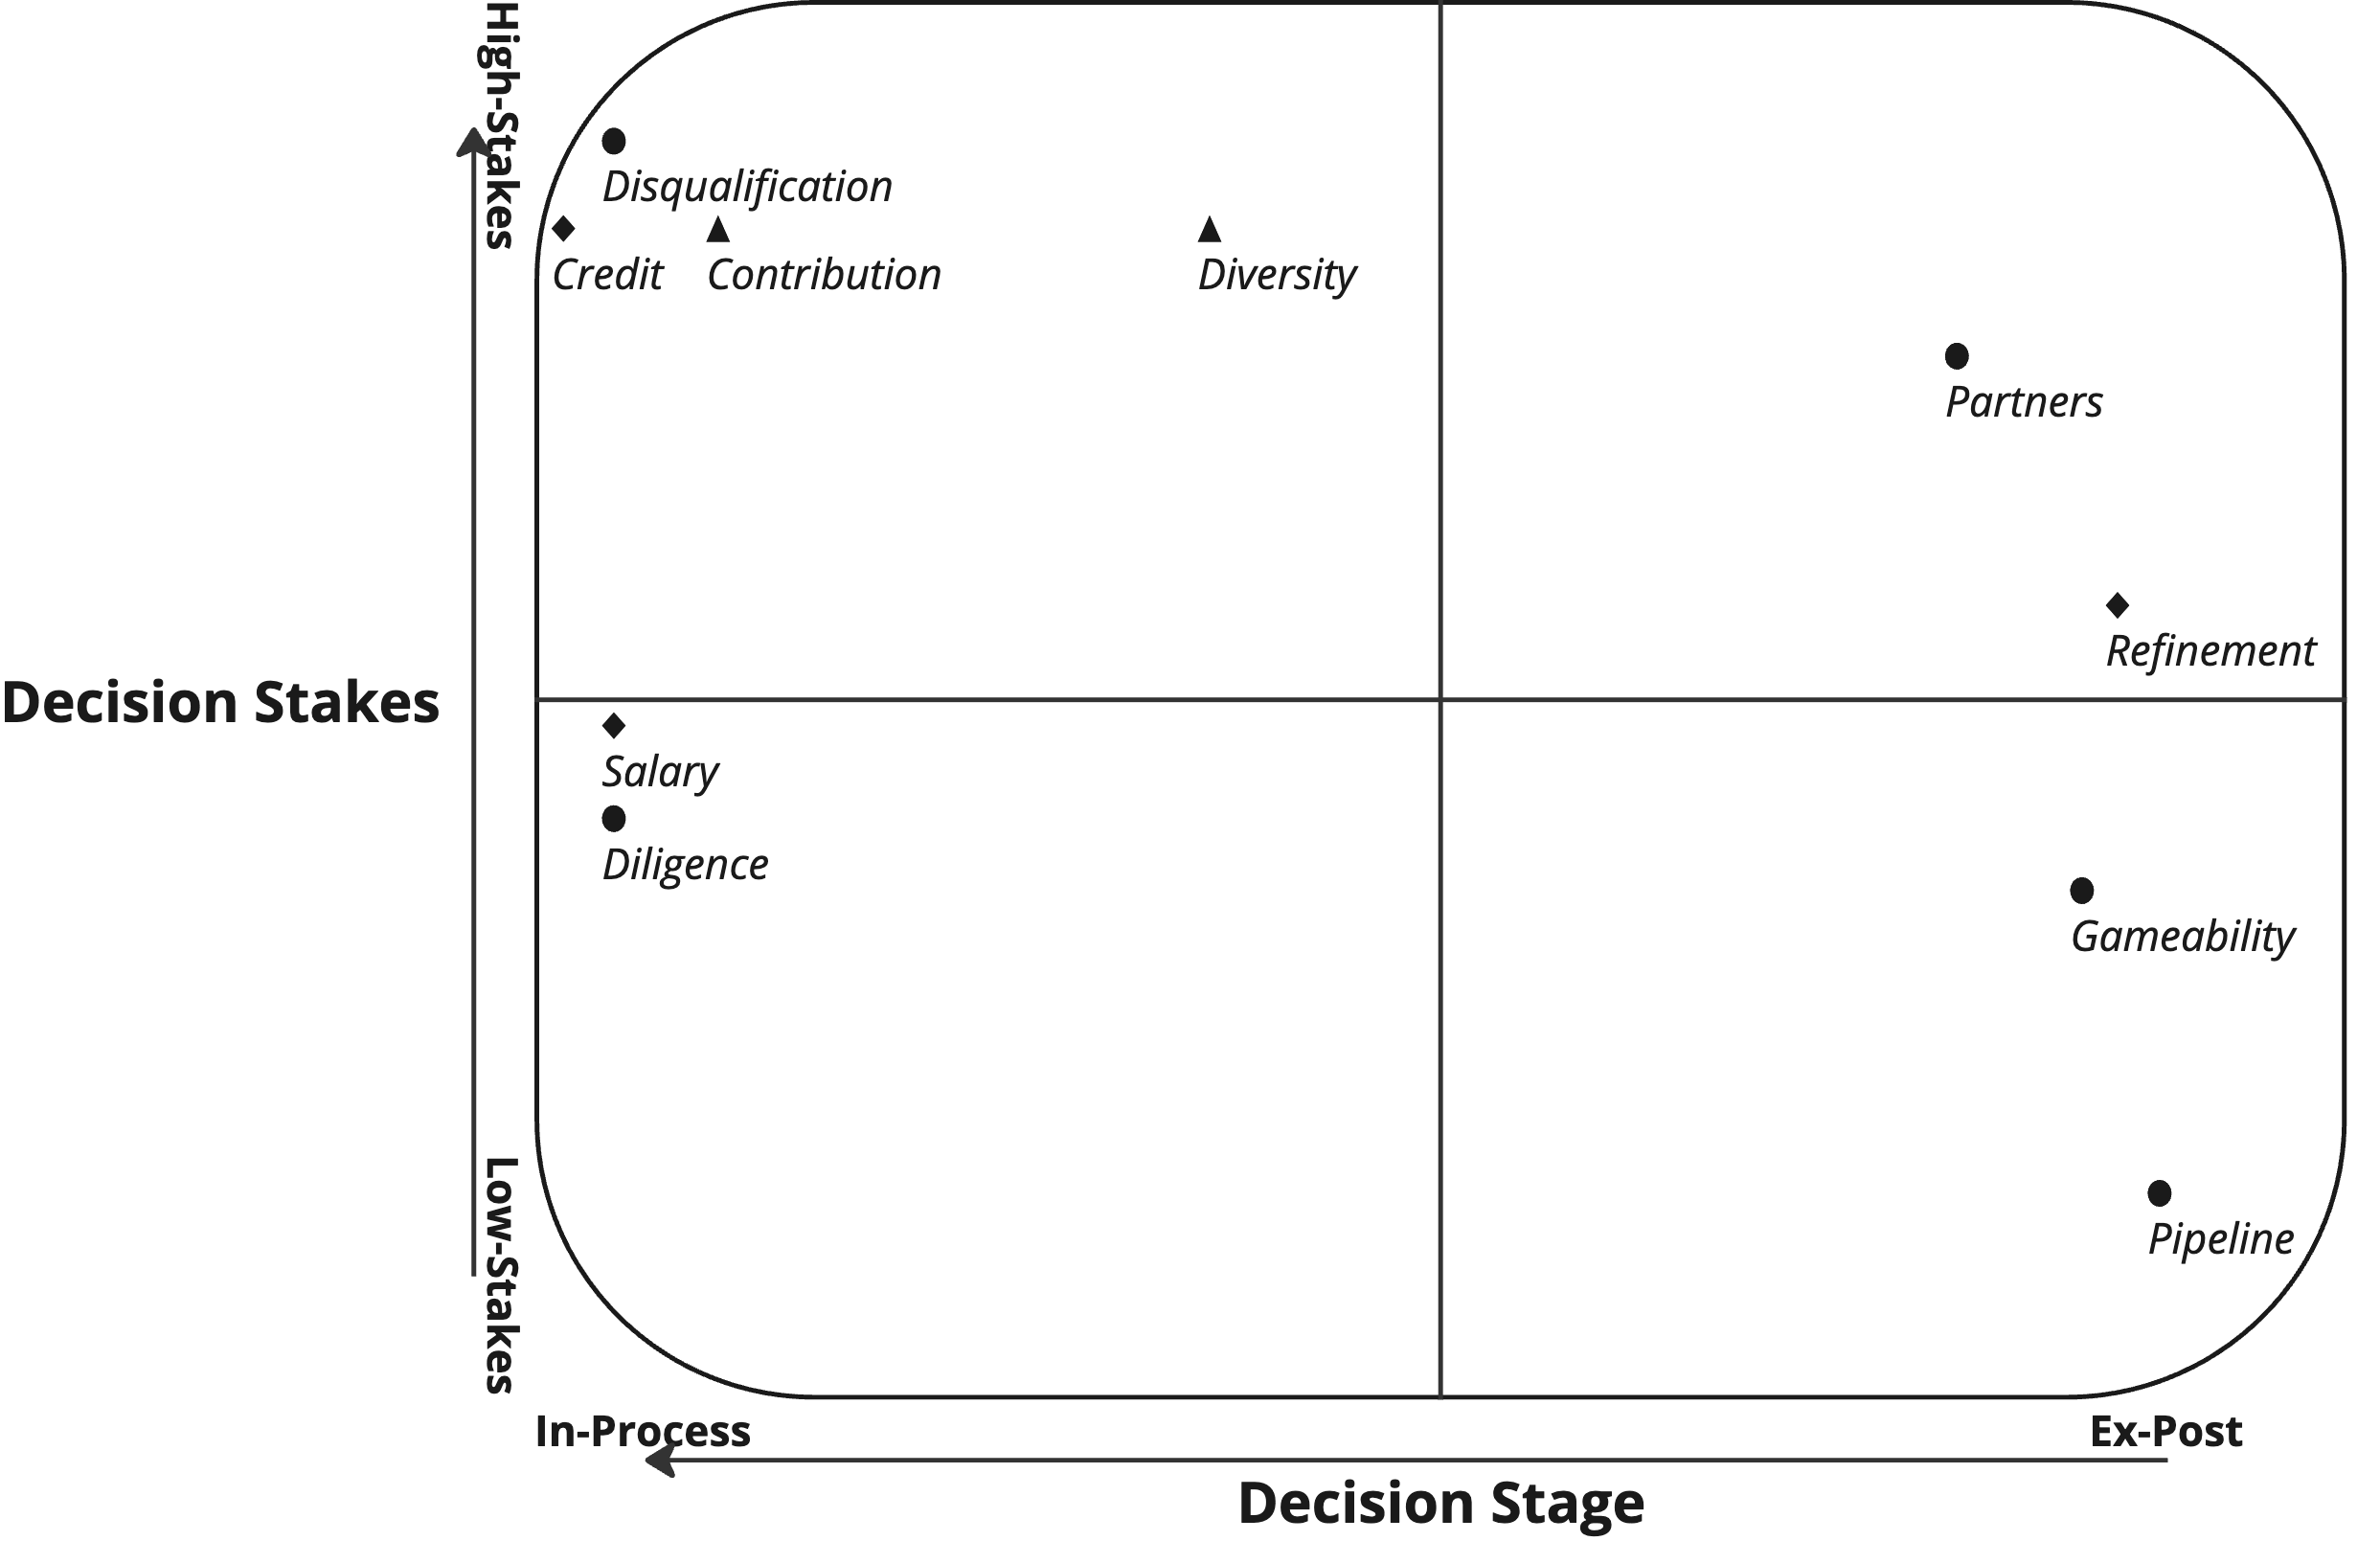
\includegraphics[width=0.8\textwidth]{context/full_decision_matrix.png}
  \caption{This figure places the decisions from Table \ref{tab:full_decision_list} on the Decision Matrix.}
  \label{fig:full_decision_matrix}
\end{figure}

\section{Programs we Work With}\label{sec:programs}
\subsection{Foreword To Section \ref{sec:programs}}
We work with two global scholarship and talent investment programs: the Ellison Scholars Program and the Rise Program. Both programs have asked that they not be identified in public facing research, and thus we request that reviewers not share details on Section \ref{sec:programs} or knowledge contained within. Throughout the remainder of this Thesis, we refer to the Ellison Scholars Program and the Rise Program as Program A and Program B, respectively. However, to provide reviewers with the context and detail required to appropriately evaluate this work, we provide a brief overview of each program in this section.

\subsection{The Rise Program}\label{ssec:rise}
\subsubsection{Program Overview}
Initiated from a $\$1$-billion investment, Schmidt Futures and the Rhodes Trust's Rise program\footnote{https://www.risefortheworld.org/} finds and selects talented and disadvantaged 15-to-17-year-olds from around the world and helps them achieve their full career and service potential. Rise supports selected `winners' and `finalists' with a variety of benefits accessible at different points in their life. We work with Rise from the program's inception in 2021 until 2024. In each of these years, Rise has made a commitment to select up to 100 winners and up to 500 finalists from their pool of applicants. In the four applications cycles between 2021 and 2024, during which time Rise has selected 400 winners and nearly 2000 finalists from hundreds of thousands of started applications.

Rise uses a flexible benefits model, where winners (and, in some cases, finalists) gain access to a variety of potential resources, but utilise only resources they demonstrate need of. For example, applicants who recieve full scholarships to their university may not recieve an academic scholarship from Rise. Program benefits include academic scholarships, educational resources and programs, networking opportunities, and even funding for winner-led startups.\footnote{As academic scholarships comprise a large portion of program benefits, we speak about Rise as a ``scholarship and talent investment'' program throughout. This is our own language, and is intended to further anonymise the program. Similarly, we replace the program-specific term ``winners'' with ``scholars''.}

\subsubsection{The Selection Process}
The program uses a two-stage selection process designed to be accessible to candidates various global and socioeconomic backgrounds. In stage one, applicants submit various application materials asynchronously; Rise selects up to 500 finalists based on the quality of those materials and the program's cohort composition goals. In stage two, finalists engage in one of several ``finalist days'' consisting of various collaborative live activities and an interview; after all finalist days are completed, Rise uses information from both stages to select 100 winners.

\begin{figure}[htbp]
    \centering
    \begin{subfigure}{.45\textwidth}
        \centering
        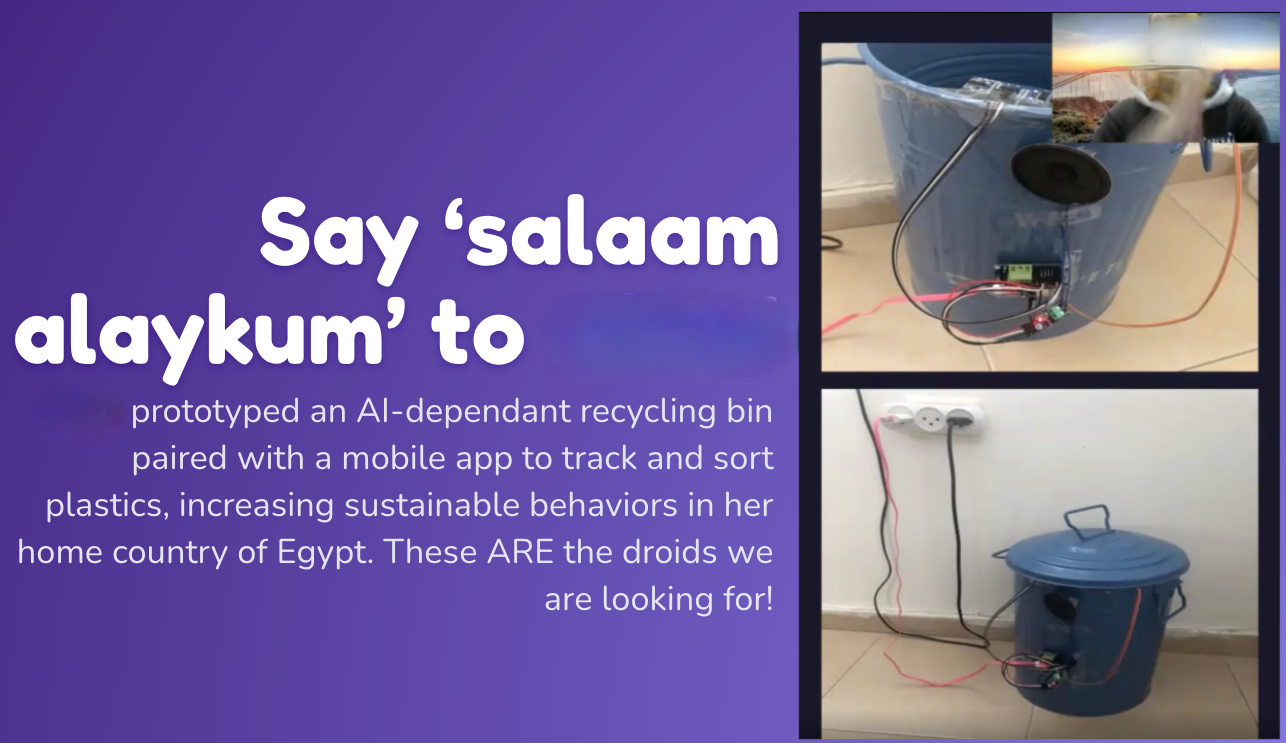
\includegraphics[width=\linewidth]{context/proj1.png}
        \caption{Sample Project 1}
        \label{sfig:can}
    \end{subfigure}
    \hfill
    \vspace{1em}
    \begin{subfigure}{.45\textwidth}
        \centering
        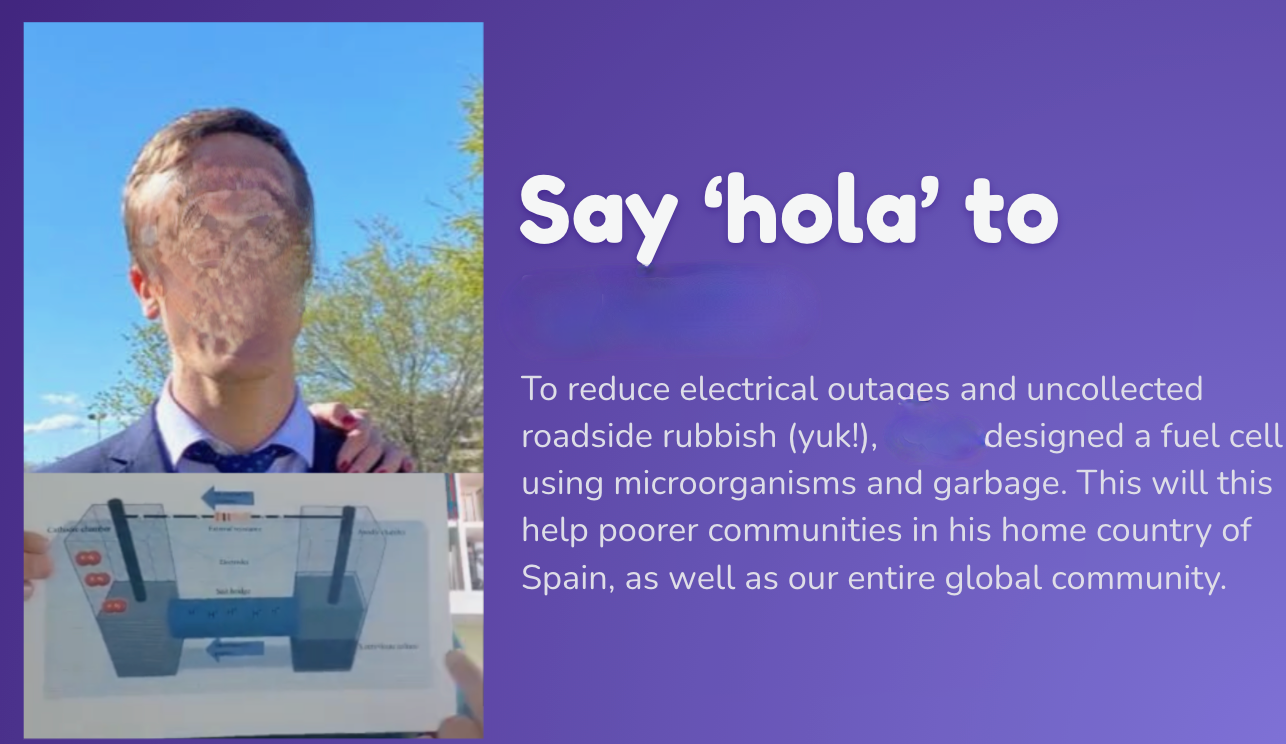
\includegraphics[width=\linewidth]{context/proj2.png}
        \caption{Sample Project 2}
        \label{sfig:cell}
    \end{subfigure}
    \hfill
    \vspace{1em}
    \begin{subfigure}{.45\textwidth}
        \centering
        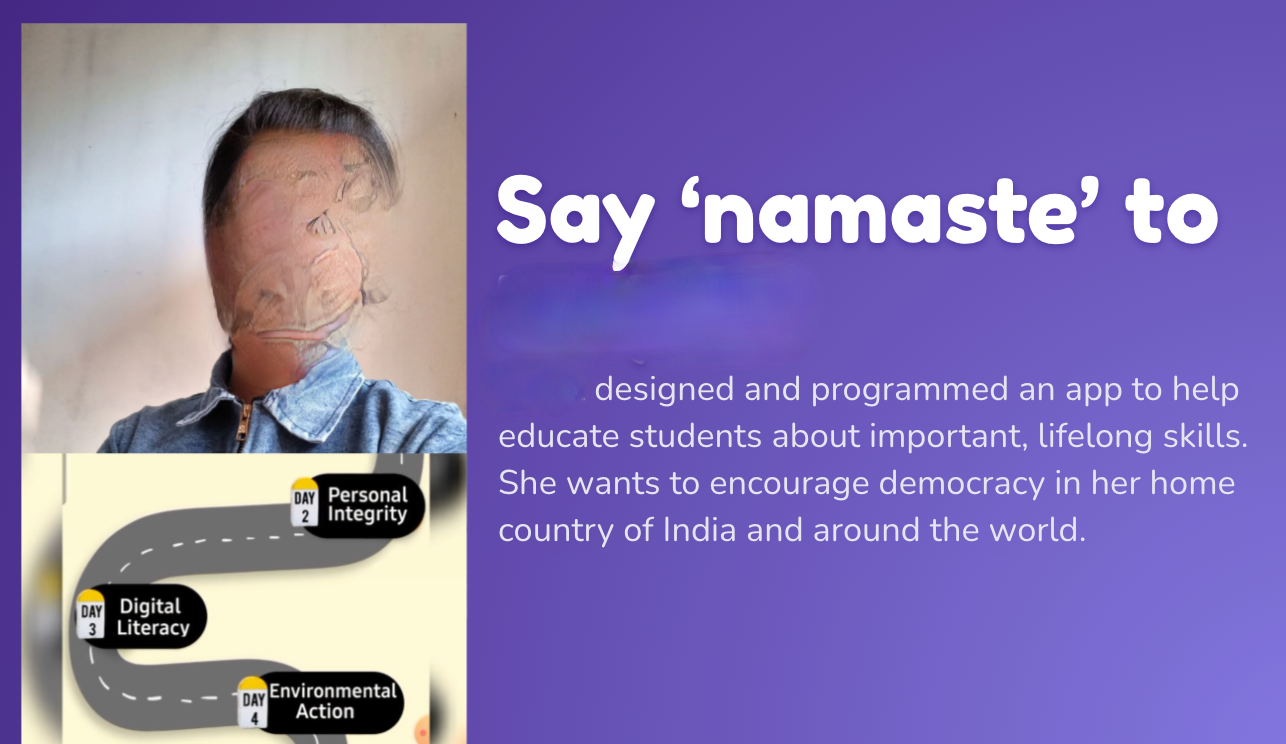
\includegraphics[width=\linewidth]{context/proj3.png} 
        \caption{Sample Project 3}
        \label{sfig:app}
    \end{subfigure}
    \caption{The three panels in this figure depict slides from a program presentation that highlighted three projects that were submitted as part of Rise's 2021 application cycle. Figure \ref{sfig:can} depicts an AI-dependent recycling bin paired with a mobile app to track and sort plastics. Figure \ref{sfig:cell} depicts schematics for a clean fuel cell using microorganisms and garbage. Figure \ref{sfig:app} depicts an app to help education students about the importance of various technical and character skills. Names have been removed and pictures blurred to de-identify program applicants.}
    \label{fig:example_projects}
\end{figure}

Stage one of selection occurs asynchronously (via smartphone, laptop, or, in rare cases, pen and paper) and in two parts. The first part requires applicants to submit an application form with their demographic information and either video or written essays. The first of these two essays explains a real-world problem the applicant wishes to solve, while the second discusses either the ways in which they consider themselves privileged or the challenges they have overcome.\footnote{Refinements to the application process between years all application materials change slightly over time. This change is most dramatic in the case of this second essay, where the focus of the essay changed from an applicant declaration of their own privilege to a description of a challenge the applicant has faced and how they overcame it. Changes appear throughout the application across years; we only detail them where it is relevant to our research.} In the second part, applicants complete a set of digital cognitive assessments and a project showcasing their talent.\footnote{In rare cases, technology or accessibility limitations prevented applicants from completing the cognitive assessment; these applicants were considered on the merits of their submitted materials.} The project showcase is a distinctive part of Rise's selection process whereby participants: (1) identify a problem they wish to solve, (2) research solutions to that problem, (3) implement those solutions, and (4) reflect on what they learned from the project. Participants submit one essay (video or text) on each of these four stages. Three example projects can be found in Figure \ref{fig:example_projects}. All applicants also submit a short written essay explaining their project and its significance. For an overview of the stage one selection design, see Figure \ref{fig:design}.

Stage two of selection occurs synchronously (though still remotely) in one of several ``finalist days''. The finalist days consist of up to five activities of three types: presentations (where finalists present information about their project), group activities (where finalists collaborate to discuss and solve problems), or interviews (where finalists are interviewed). All activities were judged by a pool of adult `selectors' who assessed finalists according to a rubric. Winner selection decisions were made based both on data collected in stage two and information retained from stage one.

\subsubsection{Data Collection}
Across the application cycle, Rise collects a variety of data from applicants. This data includes traditional merit-based measures – including cognitive tests, written essays, and referrals – as well as non-traditional measures – including peer reviewed video essays, gameified skill tests, and application platform behaviors. Many of these measures are used only for research purposes, and some are tangential to our research on supporting the selection process. We discuss relevant measures here. More detail on these measurements, especially for the 2021-2023 application cycles, can be found in Chapter \ref{ch:spf}, where findings depend on the specifics of Rise program measurement.

\paragraph{Cognitive Assessments}
Rise collects two data from two cognitive assessments taken by applicants. The first is based on the International Cognitive Assessment Resource (ICAR) \cite{condon2014international, subotic2020psychometric}, and has, in various selection cycles, incorporated four different item types: Cube Rotation, Number Sequence, Matrix Reasoning, and Verbal Reasoning. Applicants are given nonverbal and verbal sub-scores, which are using a Bayesian generalized linear item response model \cite{burkner2021bayesian}. In some cycles, only the nonverbal score was used, while other cycles combined the two to create one singular score.

The second cognitive assessment consists of a gameified skills test called Roomworld developed by the Human Information Processing (HIP) lab in the Department of Experimental Psychology at the University of Oxford.\footnote{Roomworld was created and scored by an external partner to the program and the specific scoring algorithm was not shared with the authors of this paper.}

\paragraph{Peer Review}
Stage one applicant essays were judged by two types of human evaluators: other applicants (peers) and adults with some expertise on the project topics (experts). Though \textcite{Anvari2021EffectivenessOP} provide evidence for the efficiency and effectiveness of peer review as a measurement of aptitude, peer review was (and remains) experimental \cite{Rahmatillah2022AnalyzingFA}. That said, \textcite{VanderSchee2022UsingCP} find that decision subjects of a blind peer review process experience just outcomes both according to the similar treatment and similar outcomes princples. Thus, though Rise treated peer reviews as experimental, peer scoring played an integral role in the Rise process. To collect peer reviews, each applicant was assigned to review 20 of each essay submitted. Each review consisted of Likert scale judgements designed to measure: intelligence, perseverance, empathy, integrity, sense of calling, and impact on the applicant.

\paragraph{Expert Review} 
Experts, on the other hand, were only asked to assess applicant project essays. Each reviewer was assigned a number of projects proportional to their capacity to review. Like peers, experts were asked to review different elements of the project, using Likert scales to gauge how effective the project was at accomplishing what the applicant intended and how impressive the project was relative to other projects in this field. 

\paragraph{Finalist Day Activities}
The finalist day activities were assessed by selectors through a mix of qualitative and quantitative measures. Each activity was scored on a rubric, and the scores were aggregated to create a final score for each finalist on each activity type. Additionally, selectors were given an option to provide specific qualitative feedback on applicants.

\subsection{The Ellison Scholars Program}\label{ssec:ellison}
\subsubsection{Program Overview}
Funded and administered by the Ellison Institute of Technology, The Ellison Scholars Program\footnote{https://eit.org/ellisonscholars/} is a global scholarship program that seeks to develop global technology innovators and leaders by finding and supporting talented people passionate about solving humanity’s most serious problems as they study at the University of Oxford and solve global problems through innovation. The program seeks to select at least twenty scholars each year beginning in 2025.

As the Ellison Scholarship's inaugural cohort has yet to be selected, program benefits have yet to be dispersed. However, the program has committed to providing scholars with an academic scholarship to the University of Oxford and paid internships. These internships, as well as the program as a whole, are organised around four humane endeavours: (1) Health and Medical Science, (2) Food Security and Sustainable Agriculture, (3) Climate Change and Clean Energy, and (4) Government Innovation and Era of Artificial Intelligence.

\subsubsection{The Selection Process}
As humane endeavours form a large part of the Ellison Scholarship, the selection process places special emphasis on suitability for these topics. The program has applicants declare their humane endeavours of interest and assesses applicants relative to these humane endeavours. Additionally, as the program seeks to pursue all four endeavours, diversity-like considerations require the program to ensure that scholars are chosen for each humane endeavour. However, though many selection practitioners on the Ellison Scholarship selection team are sympathetic to desires for demographic diversity, the program's theory of change does not lend itself to explicit diversity considerations (unlike Rise)

The Ellison Scholarship employs a three-stage selection process. In stage one, applicants submit various application materials asynchronously; the program selects semi-finalists based on the quality of those materials and the program's cohort composition goals. In stage two, semi-finalists apply to the University of Oxford, and the University handles their own internal selection process; program applicants who recieve Oxford scholarships are dubbed Finalists. In stage three, finalists engage in a series of synchronous activities before final decisions are made by the program's board. 

In stage one of selection, applicants submit: their demographic information; selections for humane endeavour, Oxford course, and preferred project; their education record; a list of achievements; and four written essays speaking to their suitability for the program. These essays speak to the applicant's alignment to their chosen humane endeavour, alignment to their chosen course at Oxford, and their particular skills and archetype. After submitting this application, all applicants are invited to take a cognitive assessment assessing convergent and divergent reasoning.

In stage two, semi-finalists apply to the University of Oxford; in stage three, finalists engage in a series of synchronous activities before final decisions are made by the program's board. As the Ellison Scholars program is still selecting their inaugural cohort, neither stage two nor stage three have been enacted. Thus, we omit details on them here. 

\subsubsection{Data Collection}
The Ellison institute collects and constructs a number of different aptitude measurements of applicants. This is primarily traditional merit-based measures, e.g., cognitive tests, written essays, or academic transcripts. Additionally, the program constructs a number of more experimental measures from gathered data. We discuss relevant measures here.

\paragraph{Cognitive Assessments} 
Much like the Rise program, the Ellison Scholarship uses a cognitive assessment based on the International Cognitive Assessment Resource (ICAR) \cite{condon2014international,subotic2020psychometric}. Though the details of implementation differ, both programs use the same four item types and same scoring algorithm \cite{burkner2021bayesian}.

Additionally, the Ellison Scholarship relies on a divergent thinking assessment based on Guildford's Alternative Uses Task (AUT) \cite{guilford1967creativity}. This task is chosen for its ability to measure ``divergent thinking'', i.e., creativity or innovativeness \cite{dumas_measuring_2020,organisciak_beyond_2023}. Each question is timed at roughly 90 seconds per question, and each applicant is given ten questions. Applicants are scored according to \textcite{organisciak_beyond_2023}'s Open Creativity Scoring with Artificial Intelligence (OCSAI) scoring algorithm.\footnote{https://openscoring.du.edu/}

The Ellison Scholarship combined both ICAR and AUT scores to get an overall cognitive assessment score.

\paragraph{AI-driven Assessment of Essays}
The Ellison Scholarship employs an AI-based scoring method as a preliminary screen on applicants' four written essays. The program's approach broadly follows the approach of \textcite{xiao2024humanaicollaborativeessayscoring}; the Ellison Scholars program requested that specific details of the program's implementation not be shared. After these four essays are scored, an overall AI-driven score of applicants is calculated.

\paragraph{Expert Assessment of Applications}
Stage one applicants whose test scores or AI-driven essay scores merited further consideration were judged by expert human evaluators in two types of reviews: anonymous reviews (where reviewers only had access to applicant essays, grades and achievements) and contextual reviews (where reviewers had access to supporting information such as references or applicant demographics). As compared to Rise's experts, the Ellison Institute engaged adult reviewers in a rigorous training process before qualifying them as expert reviewers.

In each review, experts judged applicants on a number of axes related to specific program goals (e.g., whether the applicant demonstrated an interest in the humane endeavour they chose). Anonymous and contextual reviews were ultimately pooled, and an overall review score was calculated.

\paragraph{Semifinalist and Finalist Assessment}
As the program is still selecting their inaugural cohort, they have yet to undergo semi-finalist or finalist assessment. We thus omit the details of these assessments from this thesis.